% !TeX program = lualatex
% ================================================================
% Polish Parallel Text Version of ProportionCrossTopics
%
% Generated by the server using the following settings:
%
%   language            Polish (pol)
%   text direction      left to right
%   font                Noto Serif
%   fallback font       Noto Serif
%   built from          latex/worksheets/ratioAndProportion/crossTopic/proportionCrossTopics.tex
%   vocabulary key      latex/worksheets/ratioAndProportion/crossTopic/proportionCrossTopics/L2/pol/proportionCrossTopics_polishKey.tex
%   tier 3 vocabulary   green   RGB 0 128 0
%   English text        black   RGB 0 0 0
%   Polish text         purple  RGB 112 48 160
%   layout macros       version 3
%
% Please don't edit any information in this comment block - the server
% compares it against the current settings and rebuilds this file when
% they differ, so changes here would be overwritten. However, feel free
% to make updates to the LaTeX below if you want to edit it.
% ================================================================

\documentclass[12pt]{article}
% ================================================================
% Copied from the English sheet this was translated from, so that
% anything it sets up for itself still works here
% ================================================================
\usepackage{amsmath} % For basic math symbols and environments
\usepackage{tikz} % For drawing shapes
\usepackage{enumitem} % For customizing lists
\usepackage[margin=1in]{geometry} % For setting page margins
\usepackage{float} % For better control of figure placement
\usetikzlibrary{shapes.geometric, arrows.meta, positioning}
\usepackage{enumitem} % For customising lists
\usepackage{siunitx} % For units


\title{Proportion Extension Problems}
\date{}

% Characters this language's font has not got are borrowed from another,
% rather than being silently dropped - see docs/translated-sheet-latex.md
\directlua{%
  if luaotfload and luaotfload.add_fallback then
    luaotfload.add_fallback("eallatinfallback",
      { "Noto Serif:mode=harf;" })
  else
    tex.error("this luaotfload is too old to register a fallback font")
  end
}
\usepackage[english]{babel}
\babelprovide[import]{polish}
\babelfont[polish]{rm}[Renderer=Harfbuzz, BoldFont={Noto Serif}, ItalicFont={Noto Serif}, BoldItalicFont={Noto Serif}, RawFeature={fallback=eallatinfallback}]{Noto Serif}
\babelfont[polish]{sf}[Renderer=Harfbuzz, BoldFont={Noto Serif}, ItalicFont={Noto Serif}, BoldItalicFont={Noto Serif}, RawFeature={fallback=eallatinfallback}]{Noto Serif}
\newcommand{\ealtext}[1]{\foreignlanguage{polish}{#1}}
\newcommand{\ealtextblock}[1]{{\raggedright\foreignlanguage{polish}{#1}\par}}
% ================================================================
% EAL layout helpers
% ================================================================
\usepackage{xcolor}

\definecolor{ealkeycolour}{RGB}{0,128,0}
\definecolor{ealenglish}{RGB}{0,0,0}
\definecolor{ealtwocolour}{RGB}{112,48,160}

\newsavebox{\ealboxen}
\newsavebox{\ealboxtr}
\newlength{\ealglosswd}
\newlength{\ealglossraise}
\setlength{\ealglossraise}{1.15em}

% a tier 3 word, in English and in translation alike
\newcommand{\ealkey}[1]{\textcolor{ealkeycolour}{#1}}
\newcommand{\ealkeytr}[1]{\textcolor{ealkeycolour}{\ealtext{#1}}}

% One translated word above one English word. Built from kernel
% primitives, never a tabular, which would break wherever the sheet
% loads array, booktabs or tabularx. The box is as wide as the wider of
% the two, so a long translation pushes its neighbours aside instead of
% overlapping them, and it claims its full height so a table row or a
% TikZ node makes room for it.
\newcommand{\ealgloss}[2]{%
  \sbox{\ealboxen}{\ealkey{#1}}%
  \sbox{\ealboxtr}{\small\textcolor{ealtwocolour}{\ealtext{#2}}}%
  \setlength{\ealglosswd}{\wd\ealboxen}%
  \ifdim\wd\ealboxtr>\ealglosswd\setlength{\ealglosswd}{\wd\ealboxtr}\fi
  \leavevmode
  \makebox[\ealglosswd][c]{%
    \makebox[0pt][c]{\usebox{\ealboxen}}%
    \makebox[0pt][c]{\raisebox{\ealglossraise}{\usebox{\ealboxtr}}}%
  }%
}

% opens up line spacing around a block of glosses, so the raised
% translations sit clear of the line above
\newenvironment{ealglossed}{\par\linespread{2.1}\selectfont\ignorespaces}{\par}

% a whole translated sentence above its English counterpart. block level,
% so it does not belong inside a tabular cell
\newcommand{\ealpara}[2]{%
  \par\addvspace{0.5\baselineskip}%
  {\color{ealtwocolour}\ealtextblock{#1}}%
  \penalty200
  {\color{ealenglish}#2\par}%
  \addvspace{0.5\baselineskip}%
}

\begin{document}

\maketitle

\section*{Direct \ealkey{Proportion} Past}

\begin{enumerate}
    \item
    \ealpara{Torebka 5 jabłek kosztuje £1.20. Jaki jest koszt o 40\% większej liczby jabłek? Ile to jabłek?}{A bag of 5 apples costs £1.20. What is the cost of 40\% more apples? How many apples is that?}
    \vspace{0.6cm}

    \item
    \ealpara{Jeśli 10\% liczby wynosi 15, to ile wynosi 40\% tej liczby?}{If 10\% of a number is 15, what is 40\% of the number?}
    \vspace{0.6cm}

    \item
    \ealpara{Sklep oferuje 15\% zniżki przy zakupie 3 takich samych przedmiotów. Jeśli jedna książka normalnie kosztuje £8, ile będą kosztować 3 książki ze zniżką?}{A shop offers a 15\% discount for buying 3 of the same item. If one book normally costs £8, how much would 3 books cost with the discount?}
    \vspace{0.6cm}

    \item
    \ealpara{Koszt paliwa jest \ealkeytr{wprost proporcjonalny} do liczby kupionych litrów. Jeśli 40 litrów kosztuje £68.00, a cena następnie wzrośnie o 5\%, ile będzie kosztować 25 litrów przy nowej cenie?}{The cost of fuel is \ealkey{directly proportional} to the number of litres purchased. If 40 litres cost £68.00, and the price then increases by 5\%, what will 25 litres cost at the new price?}
    \vspace{0.6cm}

    \item
    \ealpara{Przychód kawiarni jest \ealkeytr{wprost proporcjonalny} do liczby klientów. W poniedziałek mieli 120 klientów i zarobili £420. We wtorek podnieśli ceny o 8\%. Ilu klientów mieli we wtorek, jeśli ich przychód wynosił £453.60?}{A coffee shop's revenue is \ealkey{directly proportional} to the number of customers. On Monday, they had 120 customers and made £420. On Tuesday, they increased their prices by 8\%. How many customers did they have on Tuesday if their revenue was £453.60?}
\end{enumerate}

\vspace{1.2cm}

\newpage{}

\section*{Direct Proportion Future}

\ealpara{Instrukcje: Rozwiąż poniższe zadania dotyczące \ealkeytr{obwodu} i \ealkeytr{pola} figur 2D. Figury są \ealkeytr{podobne}, chyba że podano inaczej.}{\textbf{Instructions:} Solve the following problems involving the \ealkey{perimeter} and \ealkey{area} of 2D shapes. The shapes are \ealkey{similar} unless stated otherwise.}

\begin{enumerate}[resume]
    \item
    \ealpara{\ealkeytr{Obwód} \ealkeytr{kwadratu} jest \ealkeytr{wprost proporcjonalny} do długości jego boku. Jeśli \ealkeytr{kwadrat} o boku 4 cm ma \ealkeytr{obwód} 16 cm, jaki jest \ealkeytr{obwód} \ealkeytr{kwadratu} o boku 11 cm?}{The \ealkey{perimeter} of a \ealkey{square} is \ealkey{directly proportional} to the length of its side. If a \ealkey{square} with a side of 4 cm has a \ealkey{perimeter} of 16 cm, what is the \ealkey{perimeter} of a \ealkey{square} with a side of 11 cm?}
    \vspace{1.2cm}

    \item
    \ealpara{Długość i szerokość \ealkeytr{prostokąta} są w prostej \ealkeytr{proporcjonalności}. \ealkeytr{Prostokąt} ma długość 5 cm i \ealkeytr{obwód} 18 cm. Jaki jest \ealkeytr{obwód} \ealkeytr{prostokąta} o długości 15 cm?}{The length and width of a \ealkey{rectangle} are in a direct \ealkey{proportion}. A \ealkey{rectangle} has a length of 5 cm and a \ealkey{perimeter} of 18 cm. What is the \ealkey{perimeter} of a \ealkey{rectangle} with a length of 15 cm?}

    \begin{center}
    \begin{tikzpicture}[scale=0.7, baseline=(current bounding box.center)]
        \draw (0,0) rectangle (5, 4);
        \node[above] at (2.5, 4) {5 cm};
        \node[right] at (5, 2) {? cm};
    \end{tikzpicture}
    \end{center}
    
    \vspace{1.2cm}

    \item
    \ealpara{\ealkeytr{Pole} \ealkeytr{kwadratu} jest \ealkeytr{wprost proporcjonalne} do \ealkeytr{kwadratu} długości jego boku. Jeśli \ealkeytr{kwadrat} o boku 3 cm ma \ealkeytr{pole} 9 cm$^2$, jakie jest \ealkeytr{pole} \ealkeytr{kwadratu} o boku 7 cm?}{The \ealkey{area} of a \ealkey{square} is \ealkey{directly proportional} to the \ealkey{square} of its side length. If a \ealkey{square} with a side of 3 cm has an \ealkey{area} of 9 cm$^2$, what is the \ealkey{area} of a \ealkey{square} with a side of 7 cm?}
    \vspace{1.2cm}

    \item
    \ealpara{Dwa \ealkeytr{podobne} \ealkeytr{trójkąty} są pokazane poniżej. \ealkeytr{Obwód} mniejszego \ealkeytr{trójkąta} wynosi 21 cm. Długości boków większego \ealkeytr{trójkąta} są 2.5 razy większe niż mniejszego. Jaki jest \ealkeytr{obwód} większego \ealkeytr{trójkąta}?}{Two \ealkey{similar} \ealkey{triangles} are shown below. The \ealkey{perimeter} of the smaller \ealkey{triangle} is 21 cm. The side lengths of the larger \ealkey{triangle} are 2.5 times those of the smaller one. What is the \ealkey{perimeter} of the larger \ealkey{triangle}?}

    \begin{center}
    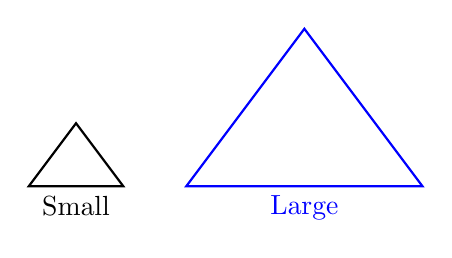
\begin{tikzpicture}[scale=0.4, baseline=(current bounding box.center)]
        % Small Triangle
        \draw[thick] (0,0) -- (3,0) -- (1.5,2) -- cycle;
        \node[below] at (1.5, 0) {Small};
        % Large Triangle
        \draw[thick, blue] (5,0) -- (12.5,0) -- (8.75,5) -- cycle;
        \node[below, blue] at (8.75, 0) {Large};
    \end{tikzpicture}
    \end{center}
    
    \vspace{1.2cm}

    \item
    \ealpara{\ealkeytr{Prostokątny} ogród ma 10 m długości i 6 m szerokości. Ma powstać nowy ogród o \ealkeytr{podobnym} kształcie. \ealkeytr{Pole} nowego ogrodu musi być o 50\% większe niż w oryginale.}{A \ealkey{rectangular} garden is 10 m long and 6 m wide. A new, \ealkey{similarly} shaped garden is to be built. The \ealkey{area} of the new garden needs to be 50\% larger than the original.}
    \begin{enumerate}[label=(\alph*)]
        \item \ealpara{Jakie jest \ealkeytr{pole} nowego ogrodu?}{What is the \ealkey{area} of the new garden?}
        \item \ealpara{Jaki jest \ealkeytr{obwód} nowego ogrodu?}{What is the \ealkey{perimeter} of the new garden?}
    \end{enumerate}
    \begin{tikzpicture}[baseline=(current bounding box.center)]
        \draw (0,0) rectangle (5, 3);
        \node[above] at (2.5, 3) {10 m};
        \node[right] at (5, 1.5) {6 m};
        \node at (2.5, -0.5) {Original Garden};
    \end{tikzpicture}
    \vspace{1.2cm}
\end{enumerate}

\section*{\ealkey{Rates of Change} Past}

\begin{enumerate}[resume]

    \item
    \ealpara{Roślina miała \SI{20}{\centi\meter} wysokości. W ciągu następnego tygodnia urosła o \textbf{5\%}. Z jaką szybkością rosła, w cm na dzień?}{A plant was \SI{20}{\centi\meter} tall. Over the next week, it grew by \textbf{5\%}. At what speed did it grow, in cm per day?}
    \vspace{0.6cm}

    \item
    \ealpara{Wanna napełnia się z \ealkeytr{wielkością ilorazową} \SI{8}{\litre\per\minute}. Korek jest lekko luźny, a woda wypływa z \ealkeytr{wielkością ilorazową}, która wynosi 2\% \ealkeytr{wielkości ilorazowej} napełniania. Jeśli wanna zaczyna być pusta, ile wody jest w niej po 10 minutach?}{A bathtub fills at a \ealkey{rate} of \SI{8}{\litre\per\minute}. The plug is slightly loose, and water drains out at a \ealkey{rate} that is 2\% of the fill \ealkey{rate}. If the tub starts empty, how much water is in it after 10 minutes?}
    \vspace{0.6cm}

    \item
    \ealpara{Wartość samochodu wynosiła \pounds 15,000. Ulega \ealkeytr{amortyzacji} (traci wartość) z \ealkeytr{wielkością ilorazową} 12\% rocznie. Wartość motocykla wynosiła \pounds 8,000 i ulega \ealkeytr{amortyzacji} z 8\% rocznie. Po 3 latach, który pojazd jest wart więcej? Uzasadnij odpowiedź obliczeniami.}{A car's value was \pounds 15,000. It \ealkey{depreciates} (loses value) at a \ealkey{rate} of 12\% per year. A motorbike's value was \pounds 8,000 and it \ealkey{depreciates} at 8\% per year. After 3 years, which vehicle is worth more? Justify your answer with calculations.}
    \vspace{0.6cm}

    \item
    \ealpara{Post w mediach społecznościowych jest szybko udostępniany. Pierwszego dnia otrzymuje 200 udostępnień. Liczba udostępnień wzrasta o 15\% każdego następnego dnia.}{A social media post is shared rapidly. On the first day, it gets 200 shares. The number of shares increases by 15\% each day after that.}
    \begin{enumerate}
        \item \ealpara{Ile udostępnień otrzymuje trzeciego dnia?}{How many shares does it get on the third day?}
        \item \ealpara{Jaka jest łączna liczba udostępnień pod koniec trzeciego dnia?}{What is the total number of shares at the end of the third day?}
    \end{enumerate}
    \vspace{0.6cm}

    \item
    \ealpara{Koszty energii fabryki wynoszą \pounds 10,000 miesięcznie. Menedżer inwestuje w nowy sprzęt, który jest o 20\% bardziej wydajny. Jednak z powodu zwiększonej produkcji fabryka pracuje teraz o 15\% więcej godzin miesięcznie, w porównaniu do 200 godzin. Oblicz nowy koszt energii na godzinę i na miesiąc, zakładając, że koszt jest \ealkeytr{wprost proporcjonalny} do liczby godzin pracy.}{A factory's energy costs are \pounds 10,000 per month. The manager invests in new equipment which is 20\% more efficient. However, due to increased production, the factory now runs for 15\% more hours each month, up from 200 hours. Calculate the new energy cost per hour, and per month, assuming cost is \ealkey{directly proportional} to running hours.}

\end{enumerate}

\section*{\ealkey{Rates of Change} Future}

\begin{enumerate}[resume]

    \item
    \ealpara{\ealkeytr{Kwadrat} ma długość boku, która rośnie z \ealkeytr{wielkością ilorazową} \SI{2}{\centi\meter\per\second}. Jakie jest \ealkeytr{tempo zmian} jego \ealkeytr{obwodu}, gdy długość boku wynosi \SI{5}{\centi\meter}?, a co z sytuacją, gdy długość boku wynosi \SI{10}{\centi\meter}? Czy \ealkeytr{wielkość ilorazowa} zależy od długości boku?}{A \ealkey{square} has a side length that is increasing at a \ealkey{rate} of \SI{2}{\centi\meter\per\second}. What is the \ealkey{rate of change} of its \ealkey{perimeter} when the side length is \SI{5}{\centi\meter}?, what about when the side length is \SI{10}{\centi\meter}? Does the \ealkey{rate} depend on the side length?}
    \vspace{0.6cm}

    \item
    \ealpara{\ealkeytr{Prostokątny} parking ma \SI{60}{\metre} długości i \SI{40}{\metre} szerokości. Ma zostać ponownie wyłożony nawierzchnią. Koszt ponownego wyłożenia nawierzchni wynosi \pounds 15 za metr \ealkeytr{kwadratowy}. Oblicz całkowity koszt.}{A \ealkey{rectangular} car park is \SI{60}{\metre} long and \SI{40}{\metre} wide. It is to be resurfaced. The cost of resurfacing is \pounds 15 per \ealkey{square} metre. Calculate the total cost.}
    \vspace{0.6cm}

    \item
    \ealpara{\ealkeytr{Kołowa} plama ropy rozprzestrzenia się. Zaczyna się od \ealkeytr{promienia} 1 m. \ealkeytr{Promień} plamy rośnie z \ealkeytr{stałą} \ealkeytr{wielkością ilorazową} \SI{0.5}{\metre\per\minute}.}{A \ealkey{circular} oil spill is spreading. It starts with a \ealkey{radius} of 1m. The \ealkey{radius} of the spill is increasing at a \ealkey{constant} \ealkey{rate} of \SI{0.5}{\metre\per\minute}.}
    \begin{enumerate}
        \item \ealpara{Oblicz \ealkeytr{wielkość ilorazową}, z jaką \ealkeytr{obwód} plamy rośnie, gdy \ealkeytr{promień} wynosi \SI{4}{\metre}. (Użyj $C = \pi D$)}{Calculate the \ealkey{rate} at which the \textbf{\ealkey{circumference}} of the spill is increasing when the \ealkey{radius} is \SI{4}{\metre}. (Use $C = \pi D$)}
        \item \ealpara{Oblicz \ealkeytr{wielkość ilorazową}, z jaką \ealkeytr{obwód} plamy rośnie, gdy \ealkeytr{promień} wynosi \SI{8}{\metre}.}{Calculate the \ealkey{rate} at which the \textbf{\ealkey{circumference}} of the spill is increasing when the \ealkey{radius} is \SI{8}{\metre}.}
        \item \ealpara{Znajdź \ealkeytr{pole} plamy po 10 minutach. (Użyj $A = \pi r^2$)}{Find the \ealkey{area} of the spill after 10 minutes.  (Use $A = \pi r^2$)}
    \end{enumerate}
    \vspace{0.6cm}

    \item
    \ealpara{Ogrodnik sadzi \ealkeytr{prostokątną} grządkę kwiatową. Długość grządki rośnie z \ealkeytr{wielkością ilorazową} \SI{1}{\metre\per\hour}, a szerokość rośnie z \ealkeytr{wielkością ilorazową} \SI{0.5}{\metre\per\hour}. W pewnym momencie długość wynosi \SI{6}{\metre}, a szerokość \SI{4}{\metre}.}{A gardener is planting a \ealkey{rectangular} flower bed. The length of the bed is increasing at a \ealkey{rate} of \SI{1}{\metre\per\hour} and the width is increasing at a \ealkey{rate} of \SI{0.5}{\metre\per\hour}. At a specific moment, the length is \SI{6}{\metre} and the width is \SI{4}{\metre}.}
    \begin{enumerate}
        \item \ealpara{Z jaką \ealkeytr{wielkością ilorazową} rośnie \ealkeytr{obwód} w tym momencie?}{At what \ealkey{rate} is the \textbf{\ealkey{perimeter}} increasing at this moment?}
        \item \ealpara{O ile wzrośnie \ealkeytr{pole} po 30 minutach? Czy uważasz, że rosło ono z \ealkeytr{stałą} \ealkeytr{wielkością ilorazową}?}{How much will the \textbf{\ealkey{area}} have increased by 30 minutes later? Do you think it grew at a \ealkey{constant} \ealkey{rate}?}
    \end{enumerate}
    \vspace{0.6cm}

    \item
    \ealpara{Dekoracyjna ścieżka jest budowana wokół \ealkeytr{prostokątnego} stawu. Staw ma \SI{10}{\metre} długości i \SI{6}{\metre} szerokości. Ścieżka ma \ealkeytr{jednostajną} szerokość $x$ metrów dookoła.}{A decorative path is being built around a \ealkey{rectangular} pond. The pond is \SI{10}{\metre} long and \SI{6}{\metre} wide. The path has a \ealkey{uniform} width of $x$ metres all the way around.}
    \begin{enumerate}
        \item \ealpara{Pokaż, że \ealkeytr{pole} ścieżki, $A$, jest dane \ealkeytr{wzorem} $A = 4x^2 + 32x$.}{Show that the \ealkey{area} of the path, $A$, is given by the \ealkey{formula} $A = 4x^2 + 32x$.}
        \item \ealpara{Jeśli ścieżka jest wybrukowana z \ealkeytr{wielkością ilorazową} \SI{0.8}{\square\metre\per\minute}, jak szeroka jest ścieżka po 20 minutach, zakładając, że jest wybrukowana na zewnątrz od \ealkeytr{prostokąta}?}{If the path is being paved at a \ealkey{rate} of \SI{0.8}{\square\metre\per\minute}, how wide is the path after 20 minutes, assuming it is being paved outwards from the \ealkey{rectangle}?}
    \end{enumerate}

\end{enumerate}

\end{document}